\section{L'analyseur de DTD}

	\subsection{Les diff�rentes classes}
	
	\begin{center}
	\begin{figure}[h]
		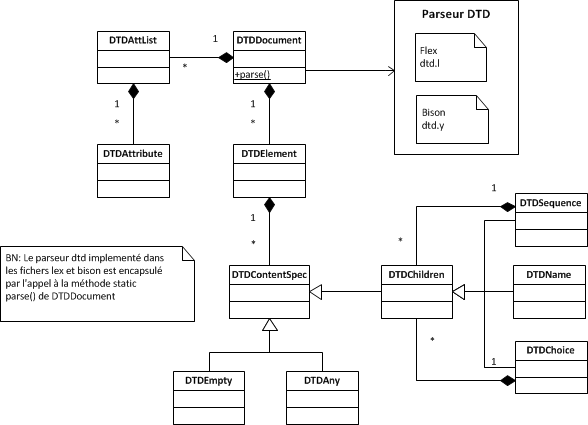
\includegraphics[width=15cm]{\PIXPATH/uml_dtd}
		\caption{Diagramme UML simplifi� de l'analyseur de DTD}
	\end{figure}
	\end{center}
	
	\subsection{Fonctionnement}
	
	\subsubsection{Parser une dtd}
	Ceci se fait par l'appel de {\tt DTDDocument::parse(const \& nomFichier )}
	L'analyseur prend en entr�e un fichier *.dtd. Il stocke ensuite
	les �l�ments et les attributs et leur contenu dans une classe
	DTDDocument.
	Le contenu d'un �l�ment est un DTDContentSpec qui peut �tre soit un DTDEmpty,
	un DTDAny ou un DTDChildren qui lui m�me peut �tre un DTDSequence, 
	un DTDName ou un DTDChoice. Lorsqu'on a un DTDChildren(DTDChoice ou 
	DTDSequence), l'appel se fait r�cursivement sur ce que celui-ci contient 
	jusqu'� DTDName qui est la seule classe ne contenant pas de DTDChildren.
	
	\subsubsection{Afficher une dtd}
	Ceci fait par l'appel de {\tt DTDDocument::display( )}
	La classe DTDDocument va afficher les informations relatives au docuement, 
	puis appelera les m�thodes display() des �l�ments et attributs qu'elle 
	contient. Eux-m�mes appeleront r�cursivement les m�thodes display() de leur
	contenus.
